\documentclass{article}
\usepackage[utf8]{inputenc}
\usepackage{natbib}
\usepackage{graphicx}
\usepackage{lipsum}
\usepackage{minted}
\usepackage{listings}
\usepackage{amsmath}
\usepackage{fixltx2e}

\title{Name Entity Recognition \\
    Project Report\\
    CS263 Data And Knowledge Bases\\\\}
\author{by\\ Magnus Settemsli Mogstad and John-Olav Storvold
\\\\\\\\\\\\\\\\\\\\\\\\\\\\\\\\\\\\\\\\\\\\\\\\\\\\\ }
\date{December 2014}



\begin{document}
\pagenumbering{gobble}
\maketitle
\clearpage
\tableofcontents
\listoftables 
\clearpage

\pagenumbering{arabic}
\section{Abstract}
For the project in CS263 data and knowledge bases we choose to look closer at a name entity recognition(NER) system, we choose this because we thought that it sounded like a interesting project and it whould teach us more about machine learning techniques\\
The meaning of a name entity regognition system is to classify words into different entitys we choose to classify on the entitys Organization, Location, Time, Person and Other. To solve this problem we approached the problem using the viterbi algorithm, which uses a hidden markov moddel to find the given states entites probability based on the previous states. With the name enitity recognition system we aim to answer which kind of entity each word is.

\section{Introduction}
At the beginning of the project we looked into making the name entity recognition system using a sequence model, which the NER system made at Stanford is using we wanted to use this because after some reading we thought it would give us the best final result. But after reading paper after paper we did not find any good description on how to implement it. Then after some consideration we found the viterbi algorithm and started to implement it in java, the viterbi algorithm uses hidden Markov Model to find the highest probability of a words entity given by the previous states. By using the viterbi algorithm and hidden Markov Model we aim to find different words entity, the different entities we aim to find is other, organization, time, location and person.

\section{Background}
To make the name entity recognition system we ended up using the viterbi algorithm and hidden Markov Model, The data we need to make from the training set is a start probability, emission probability and a transition matrix. By using these probabilities we can use the hidden Markov Model to find the highest probability of a word being a any of the five entities other, organization, time, location and person we aim to classify. The aim is to get the algorithm working before we start to find or make training sets, this is because we think the hardest part of the project is to make the algorithm work as good as we hope to make it. To check the algorithm is working we will only be using a small training set which we have created, because we used such a small data set the first results we got was not good. But then we made a program which helped us to classify other texts into training data sets, an important thing to remember when making a training set is that it should be built up by sentences because it will improve your probability to make the right classification of a word. We hope to get a success probability around 80 \% for our name entity recognition system.


\section{Body of report}
At the start of the project we looked closer at doing a sequence model name entity recognition system, but after reading papers for a couple of weeks and turning up empty in the search for an algorithm to follow. Then we choose to chase down the hidden Markov Model approach to name entity recognition, after some paper reading we ended up using the viterbi algorithm.

\subsection{Training Data Set}
To start the project we first made the file to read the words and their entity from the training data sets, the training data sets needs to be built by sentences where every word has they entity after it. This means that the data in the text files can be written in two different ways. Either you can have one word and its entity in one line, or you can have multiple words and their entity in one line see figure \ref{fig:trainingData}. Our training data set looks like the dataset you see on the right hand side of the figure, it also contains 2518 classified words which we have classified our self. This means that some words in the training data may have one or more entitie like New which is a location when it is in context with New York or it may be other when it is just by itself.

\begin{figure}[here]
\centering
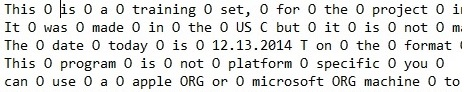
\includegraphics[width=0.78\textwidth]{fig/fig2Rapport.jpg}
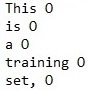
\includegraphics[width=0.2\textwidth]{fig/fig3Rapport.jpg}
\caption{Two ways to write training data set}
\label{fig:trainingData}
\end{figure}

We have made a enum java class which holds the different entities we are classifying, and in the file which reads in the training data set we use both hashmap and arraylists to keep track of the words and their entity, some of the lists we make look redundant and maybe some of them are but we did not have time to optimize and clean the code due to our poor start of the project.

\subsection{Viterbi}
When the reading of the training data set is done and all the data is in hashmaps or arraylists, we started with the viterbi algorithm. This algorithm uses the start probability, emission probability matrix and transmission probability matrix in the hidden Markov Model to find the best probability for a words entity.

\subsubsection{Guava}
Guava is a project by Google and contains some of their core libraries, for our project we are using the collections part in guava which Google have created and use. This makes it easier to store the different values in the emission and transmission probability matrix. The data structure we used is called Table and value3 is given by the values in value1 and value2.
\begin{minted}{Java}
Table<value1, value2, value3> table = HashBasedTable.create();
table.row(value1); //returns a mapping of the different value2 to value3
table.column(value2); //returns a mapping of the different value1 to value3
table.get(value1,value2); //returns value3
\end{minted}
We found this library most useful because we needed a good way to storing a probability which is decided by two variables, and it is used in both the emission, transmission probability matrix and the hidden Markov Model to store the updated values for each step.

\subsubsection{Start probability}
To find the start probability we need to find the entity of the starting word in each sentence. And then divide this entities number by the total of sentences.\\
\begin{equation}
\text{Start probability} = \frac{\text{number of start words with entity}}{\text{Toal number of sentences}}
\end{equation}
This means that the start probability will look like this\\
Entities = \{Other, Organization, Person, Time, Location\}
\begin{table}[here]
\centering
\begin{tabular}{|c|c|c|c|c|}
\hline
Other & Organization & Person & Time & Location\\
\hline
$\frac{6}{12}$ & $\frac{1}{12}$ & $\frac{2}{12}$ & $\frac{1}{12}$ & $\frac{2}{12}$\\
\hline
\end{tabular}
\caption{Start probability}
\label{tab:startProbability}
\end{table}

\subsubsection{Emission probability matrix }
The emission probability matrix is the probability of a specific word being a specific entity. If you look at table \ref{tab:emissionProbability} and the word Obama it has the probability of $\frac{1}{15}$ for person and zero for every other entity, this means that the word Obama is most likely a person.
\begin{equation}
\text{Emission probability} = \frac{\text{number of specific word with entity}}{\text{Number of words with that entity}}
\end{equation}
\clearpage
This means that the emission probability matrix will look like this only much bigger because you have to calculate the probability for each distinct word. To make this emission probability matrix we use the Table data structure from Google's guava library.
\begin{table}[here]
\centering
\begin{tabular}{|c|c|c|c|c|c|c|c|}
\hline
& Hi & This & Is & Obama & From & France & ...\\
\hline
Other & $\frac{1}{15}$ & $\frac{2}{15}$ & $\frac{1}{15}$ & $\frac{0}{15}$ & $\frac{1}{15}$ & $\frac{0}{15}$ & $\frac{2}{15}$\\
\hline
Organization & $\frac{0}{15}$ & $\frac{0}{15}$ & $\frac{0}{15}$ & $\frac{0}{15}$ & $\frac{0}{15}$ & $\frac{0}{15}$ & $\frac{0}{15}$\\
\hline
Person & $\frac{0}{15}$ & $\frac{0}{15}$ & $\frac{0}{15}$ & $\frac{1}{15}$ & $\frac{0}{15}$ & $\frac{0}{15}$ & $\frac{0}{15}$\\
\hline
Time & $\frac{0}{15}$ & $\frac{0}{15}$ & $\frac{0}{15}$ & $\frac{0}{15}$ & $\frac{0}{15}$ & $\frac{0}{15}$ & $\frac{0}{15}$\\
\hline
Location & $\frac{0}{15}$ & $\frac{0}{15}$ & $\frac{0}{15}$ & $\frac{0}{15}$ & $\frac{0}{15}$ & $\frac{1}{15}$ & $\frac{0}{15}$\\
\hline
\end{tabular}
\caption{Emission probability}
\label{tab:emissionProbability}
\end{table}

\subsubsection{Transmission probability matrix }
The Transmission probability matrix is the probability that a word is followed by a word with a given entity, if you have a word Hi then the probability tells you that the next word this is most likely a word of the entity Other(look at table \ref{tab:Transmissionprobability}).
\begin{equation}
\resizebox{.9\textwidth}{!}{
$
\text{Transmission probability} = \frac{\text{Number of words from first entity to  second entity}}{\text{Total number of first entity in text}}
$
}
\end{equation}
The transmission probability matrix is in this case 5*5(number of entities*number of entities), this is because it shows the probability of the next word in a sentence being given the current words entity.
To make this transmission probability matrix we use the Table data structure from Google's guava library.
\begin{table}[here]
\centering
\begin{tabular}{|c|c|c|c|c|c|}
\hline
& Other & Organization & Person & Time & Location\\
\hline
Other & $\frac{11}{15}$ & $\frac{1}{15}$ & $\frac{1}{15}$ & $\frac{1}{15}$ & $\frac{1}{15}$ \\
\hline
Orgainization & $\frac{1}{2}$ & $\frac{0}{2}$ & $\frac{0}{2}$ & $\frac{0}{2}$ & $\frac{0}{2}$ \\
\hline
Person & $\frac{1}{1}$ & $\frac{0}{1}$ & $\frac{0}{1}$ & $\frac{0}{1}$ & $\frac{0}{1}$ \\
\hline
Time & $\frac{2}{2}$ & $\frac{0}{2}$ & $\frac{0}{2}$ & $\frac{0}{2}$ & $\frac{0}{2}$ \\
\hline
Location & $\frac{1}{2}$ & $\frac{1}{2}$ & $\frac{0}{2}$ & $\frac{0}{2}$ & $\frac{0}{2}$ \\
\hline
\end{tabular}
\caption{Transmission probability}
\label{tab:Transmissionprobability}
\end{table}

\subsubsection{Hidden Markov Model}
We started by looking into the Baum-Welch algorithm but did not quite understand how we where to implement it, so we went with the viterbi version of hidden Markov Model.
To calculate the probability for each words entity in a sentence we are using a hidden Markov model, the hidden Markov model uses the start probability, emission probability and the transmission probability as input to calculate the entities for each word in a sentence. It does so by using the statistics created by the training data set, the training data set also contains sentences from the real world which means that the algorithm is trained to learn how a sentence is built up by specific words and entity sequences.
Since the hidden Markov model is sentence based in our project the first word in every sentence is a special case the start probability of a word is given by this. Note that no of the probability�s can be 0 it should be 0.0000000001 instead when you take the logarithm of it because you will get negative infinity if you take log\textsubscript{2} of 0 then and you will get the wrong classification.
\begin{equation}
\resizebox{0.9\textwidth}{!}{
$
P\textsubscript{entity}(word,1) = \log\textsubscript{2}(startProbFor(Entity)) - \log\textsubscript{2}(emissionprobability(Word))
$
}
\end{equation}
The words entity is decided by the entity which gives the highest value, or the entity which gives the lowest negative number in our case.\\
To get the entities for the rest of the words in the sentence, we need to use the words earlier in the sentence entities. Based on the previously entities we need to find the entity path with the highest overall probability, to get the next words entity you use this equation:
\begin{equation}
\begin{split}
P\textsubscript{entity}(word,n)=P\textsubscript{emission}(Word,entity)+\\max(P\textsubscript{entity}(word,n-1)+P\textsubscript{transmission}(entity,sameEntity),\\P\textsubscript{otherEntity}(word,n-1)+P\textsubscript{transmission}(entity,otherEntity))
\end{split}
\end{equation}
In our case the max function will have many more values, we will also have to calculate this probability for every entity we are trying to classify.
\begin{table}[here]
\centering
\begin{tabular}{|c|c|c|c|c|}
\hline
 &  Hi & Apple & Santa Barbara & Project\\
\hline
Other & \textbf{-1.2} & -2.567 & -3.455 & \textbf{-1.33}\\
\hline
Organization & -2.34 & \textbf{-1.98} & -3.45 & -3.44\\
\hline
Location & -2.33 & -4.55 & \textbf{2.33} & -4.55\\
\hline
Person & -3.21 & -3.42 & -3.34 & -7.55\\
\hline
Time & -4.33 & -4.22 & -4.12 & -8.34\\
\hline
\end{tabular}
\caption{Table of words entity with hidden markov model}
\label{tab:Table of words entity with hidden markov model}
\end{table}
The table \ref{tab:Table of words entity with hidden Markov model} shows how it chooses which entity each word should have the entity with the highest probability is bold to show how the entity path is trough a sentence.

\subsection{Result}
Our result is a name entity recognition system which identifies the different words entity based on previously words entity the sentence, by hidden Markov model which bases the decisions on the start, emission  and transmission probability.\\
By using regex expressions we have tried to help the system identify the correct entity for the different words, we only use the regex expressions to help us when the viterbi algorithm gives a word enity other. This is because when the algorithm gives the enitity other it is because it is the entity which most often occur in texts the regex expressions we have made should help us to identify time, persons and countries. 

\subsection{Statistics}
The statistics show both the error and correctness rate of our implementation of the viterbi algorithm.
\begin{equation}
\text{correct rate} = \frac{\text{number of correct}}{\text{total number of words}}
\end{equation}
\begin{equation}
\text{error rate} = \frac{\text{number of wrong entities}}{\text{total number of words}} = 1-\text{Correct rate}
\end{equation}

\begin{table}[here]
\centering
\begin{tabular}{|c|c|c|c|c|}
\hline
 & Article 1 & Article 2 & Article 3 & Article 4\\
\hline
Correct rate & 0.841 & 0.902 & 0.846 & 0.880  \\
\hline
Error rate & 0.159 & 0.098 & 0.154 & 0.120 \\
\hline
\end{tabular}
\caption{Correct and Error rate from first run}
\label{tab:Correct and Error rate from first run}
\end{table}
By looking at the correct and Error rate we can see that we are 

\section{Evaluation}
We strongly agree that we should have made the choice to either ask for the teaching assistants help og to make the switch from the sequence modeling approach to name entity recognition, because we found that the time frame was a bit short when we started working on the code for the project so late. Due to the late start we did not have so much time to tweak the algorithm and program for better performance. We could also have asked for the teaching assistants help but we thought we could find a solution to the problems we had finding a good description for sequence modeling. We could also probably have made a cleaner code but since we experienced trouble with the time we prioritized to get the system up and running and working as it should.

\section{Conclusion}
We have learned a lot about how to use a hidden Markov model to help us find highest probability based on earlier observations. We have also learned that you should ask for help if you are stuck with a problem and can not get started with a project within reasonable time, it only leads to long nights before the delivery date. The program can be improved more by getting more training data sets and make some more models which is run on the text to classify and maybe use a cross checking between the results and find the most likely entity based on the results. You can also improve the program by improving on the regex results and how to set the probability when a word gives a true value on regex queries.

\section{Bibliography}
\begin{thebibliography}{9}
\bibitem{Stanford Named Entity Recognizer}
Stanford Named Entity Recognizer
\\\texttt{http://nlp.stanford.edu/software/CRF-NER.shtml}

\bibitem{Viterbi}
Sudha Morwal, Nusrat Jahan and Deepti Chopra
\textit{Named Entity Recognition using Hidden Markov Model (HMM)}
International Journal on Natural Language Computing (IJNLC) Vol. 1, No.4, December 2012
\\\texttt{http://airccse.org/journal/ijnlc/papers/1412ijnlc02.pdf}

\bibitem{Guava}
Guava from google
\\\texttt{https://code.google.com/p/guava-libraries/}

\bibitem{Baum-Welch algorithm}
Baum-Welch algorithm
\\\texttt{http://en.wikipedia.org/wiki/Baum-Welch\char`_algorithm}

\bibitem{Chinese NER}
Jie Liu 
\textit{Chinese named entity recognition algorithm based on the improved hidden Markov model}
School of Mathematics and Computer Science, Shaanxi University of Technology, Hanzhong, Shaanxi, China
\\\texttt{http://jocpr.com/vol6-iss7-2014/JCPR-2014-6-7-1474-1478.pdf}

\bibitem{SequenceModelNER}
Dan Jurafsky, Christopher Manning
\textit{Stanford Natural Language Processing}
\\\texttt{https://class.coursera.org/nlp/lecture/59}
\end{thebibliography}

\section{Program Listings}
To run this name entity recognition system you will need a IDE like eclipse, and you will also need to import the libraries guava-18.0.jar and jsoup-1.8.1.jar(you will get these jar files when you download the project from github\\
https://github.com/johnolos/classify or when you receive it).\\
To use the imported libraries follow these steps(in eclipse):\\
1. Import project to IDE\\
2. Right click on project in package explorer\\
3. Click on build path $\rightarrow$ Configure build path\\
4. Then click button called import external jar(s)\\
5. Go to folder with project\\
6. Click on jars called guava-18.0.jar and jsoup-1.8.1.jar and click add.\\
7. Program should now be working.
\clearpage

\section{Appendix}
\begin{figure}[here]
\centering
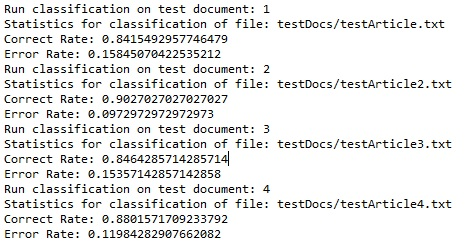
\includegraphics{fig/firstRun.jpg}
\caption{Print Screen from first run}
\label{fig:Print screen from first run}
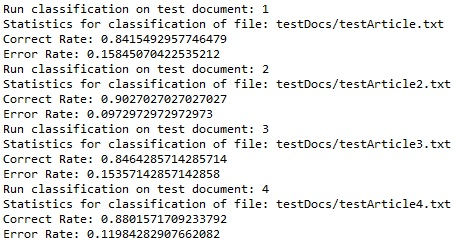
\includegraphics{fig/secondRun.jpg}
\caption{Print screen from second run}
\label{fig:Print screen from second run}
\end{figure}
As you can see from figure \ref{fig:Print screen from first run} and \ref{fig:Print screen from second run} the results are the same in both runs.




\end{document}

\introduction
This is one of the most important components of the report. It should begin with a clear statement of what the project is about so that the nature and scope of the project can be understood by a lay reader. It should summarise everything you set out to achieve, provide a clear summary of the project's background, relevance and main contributions. The introduction should set the context for the project and should provide the reader with a summary of the key things to look out for in the remainder of the report. When detailing the contributions it is helpful to provide pointers to the section(s) of the report that provide the relevant technical details. The introduction itself should be largely non-technical. It is useful to state the main objectives of the project as part of the introduction. However, avoid the temptation to list low-level objectives one after another in the introduction and then later, in the evaluation section (see below), say reference to like "All the objectives of the project have been met...".

\Background
The background section of the report should set the project into context and give the proposed layout for achieving the project goals. The background section can be included as part of the introduction but is usually better as a separate chapter, especially if the project involved significant amount of ground work. When referring to other pieces of work, cite the sources where they are referred to or used, rather than just listing them at the end.

\bodyOfReport
The central part of the report usually consists of three or four chapters detailing the technical work undertaken during the project. The structure of these chapters is highly project dependent. They can reflect the chronological development of the project, e.g. design, implementation, experimentation, optimisation, evaluation etc. If you have built a new piece of software you should describe and justify the design of your program at some high level, possibly using an approved graphical formalism such as UML. It should also document any interesting problems with, or features of, your implementation. Integration and testing are also important to discuss in some cases. You need to discuss the content of these sections thoroughly with your supervisor.

\Evaluation
Be warned that many projects fall down through poor evaluation. Simply building a system and documenting its design and functionality is not enough to gain top marks. It is extremely important that you evaluate what you have done both in absolute terms and in comparison with existing techniques, software, hardware etc. This might involve quantitative evaluation and qualitative evaluation such as expressibility, functionality, ease-of-use etc. At some point you should also evaluate the strengths and weaknesses of what you have done. Avoid statements like "The project has been a complete success and we have solved all the problems asssociated with ...! It is important to understand that there is no such thing as a perfect project. Even the very best pieces of work have their limitations and you are expected to provide a proper critical appraisal of what you have done.

\Bibliography
This consists of a list of all the books, articles, manuals etc. used in the project and referred to in the report. You should provide enough information to allow the reader to find the source. In the case of a text book you should quote the name of the publisher as well as the author(s). A weakness of many reports is inadequate citation of a source of information. It's easy to get this right so there are no excuses. Each entry in the bibliography should list the author(s) and title of the piece of work and should give full details of where it can be found.

\Conclusion
The project's conclusions should list the things which have been learnt as a result of the work you have done. For example, "The use of overloading in C++ provides a very elegant mechanism for transparent parallelisation of sequential programs". Avoid tedious personal reflections like "I learned a lot about C++ programming..." It is common to finish the report by listing ways in which the project can be taken further. This might, for example, be a plan for doing the project better if you had a chance to do it again, turning the project deliverables into a more polished end product.